\chapter{FoodOn}

\section{Ontologia}
\index{Ontologia}

La necessit� di rappresentare la conoscenza del cibo � fondamentale per molte attivit� umane tra cui agricoltura, medicina, ispezione della sicurezza alimentare, modelli di acquisto e sviluppo sostenibile.
FoodOn � una risorsa ontologica completa e open-source composta da sfaccettature gerarchiche di termini che comprendono ingredienti di base delle materie prime alimentari, termini di processo per l'imballaggio, la cottura e la conservazione e una variet� di schemi dei tipi di prodotto di livello superiore in base ai quali i prodotti alimentari possono essere classificati.
\begin{figure}[!h]
    {\begin{center}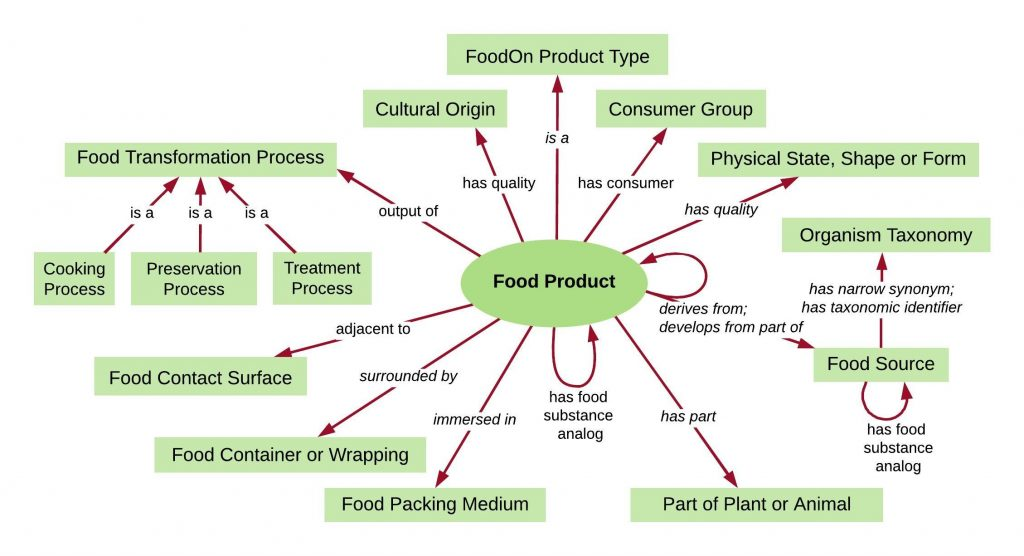
\includegraphics[width=14cm]{FIGURE/figure-1-foodon-food-schema-2-1024x556.jpeg}\end{center}}
\caption{\textbf{Diagramma di ``Food Product"} - Lo schema dei prodotti alimentari di FoodOn deriva principalemnte dalle sfaccettature della descrizione degli alimenti di LanguaL con l'aggiunta di relazioni ontologiche tra un prodotto alimentare e le relative qualit� descrittive, componenti e processi. \label{tab1}}
\end{figure}
Ad ora FoodOn � fornito sotto forma di Web Ontology Language (OWL) tramite repository GitHub del progetto stesso: \href{https://github.com/FoodOntology/foodon}{\textit{\underline{github.com/FoodOntology/foodon}}}\\


L'ultima versione pu� anche essere esplorata tramite servizi di ricerca ontologica come:
\begin{itemize}
\item BioPortal, \href{https://bioportal.bioontology.org}{\textit{\underline{bioportal.bioontology.org}}}
\item European Bioinformatics Institute Ontology Lookup Service (EMBL-EBI), \href{https://www.ebi.ac.uk/ols/}{\textit{\underline{www.ebi.ac.uk/ols/}}}
\item Ontobee, \href{http://ontobee.org}{\textit{\underline{ontobee.org}}}
\item AgroPortal, \href{http://agroportal.lirmm.fr/}{\textit{\underline{agroportal.lirmm.fr}}}
\end{itemize}
  
\subsection{FoodOn e LanguaL}
\index{FoodOn e LanguaL}
Come gi� accennato gran parte del vocabolario principale di FoodOn deriva dalla trasformazione di LanguaL, un dizionario di indicizzazione degli alimenti maturo e popolare.
In questa sezione si affronteranno le varie similitudini e differenze tra il nuovo e il vecchio progetto.
\subsubsection{Similitudini}
\index{Similitudini}
\subsubsection{Differenze}
\index{Differenze}

\section{Struttura}
\index{Struttura}
Il progetto � compatibile con Basic Formal Ontology (BFO), il che significa che tutte le classi fornite da FoodOn sono organizzate in classi BFO.
In realt� FoodOn include BFO, quindi quando si esplora l'ontologia in maniera top-down � un po' pi� complicato notare dove finisce BFO e dove inizino i termini di FoodOn.
%Le ontologie compatibili con BFO sono disponibili su \href{http://obofoundry.org/}{\textit{\underline{OBOFoundry.org}}}
Di seguito saranno mostrate le principali classi di FoodOn.\\


``\textbf{food material}" � un tipo di ``\textbf{environmental material}" che � stato posizionato sotto ``\textbf{fiat object part}" perch� il confine tra materiali ambientali adiacenti pu� essere difficile da definire fisicamente e questo si ripercuote anche su parti commestibili e non di entit� alimentari. \textit{(Figura \ref{fig:food_material})}
\begin{figure}[!h] {
	\begin{center}
		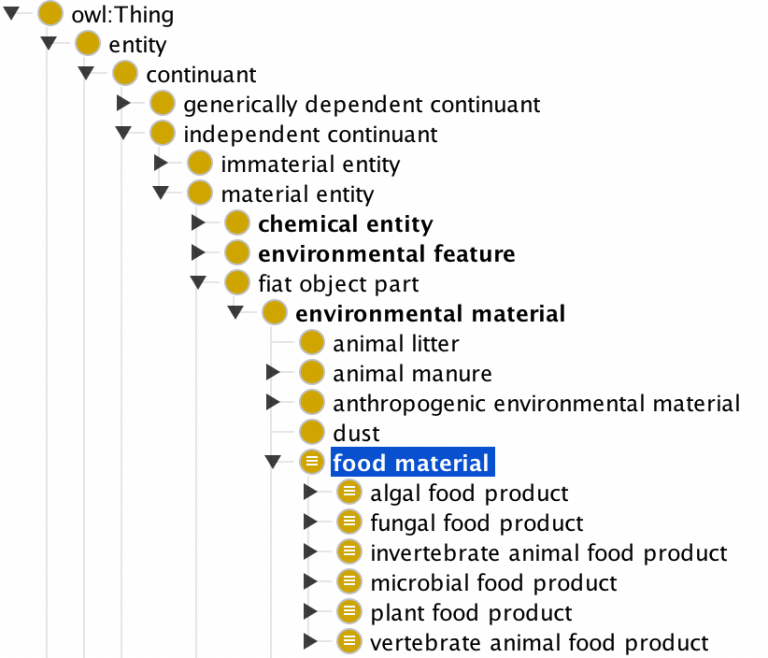
\includegraphics[width=12cm]{FIGURE/food_material-768x658.png}
	\end{center}
}
\caption{food material}
\label{fig:food_material}
\end{figure}

\newpage

Altre classi chiave di FoodOn come quelle legate a contenitori di cibo, involucri alimentari, mezzi di imballaggio, struttura della pianta, gruppi di consumatori e sostanze chimiche costituenti si trovano sotto la classe ``\textbf{material entity}". \textit{(Figura \ref{fig:material_entity})}
\begin{figure}[!h] {
	\begin{center}
		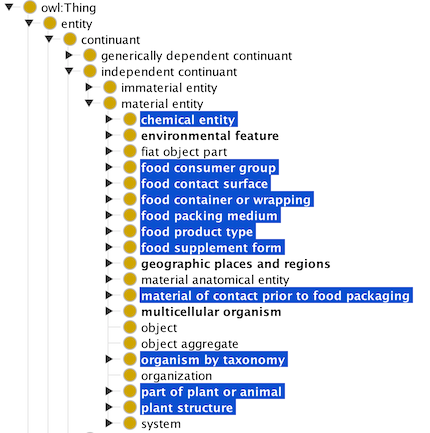
\includegraphics[width=12cm]{FIGURE/foodon_facets2.png}
	\end{center}
}
\caption{material entity}
\label{fig:material_entity}
\end{figure}

\newpage

La gerarchia ``\textbf{food product type}" contiene la principale gerarchia di FoodOn: ``\textbf{foodon product type}". ``\textit{food product type}" contiene oltre 9600 prodotti alimentari, nonch� schemi di classificazione alimentare internazionale, europea e americana di livello superiore che verranno infine associati alle categorie di ``\textit{foodon product type}". \textit{(Figur \ref{fig:food_product_type})}
\begin{figure}[!h] {
	\begin{center}
		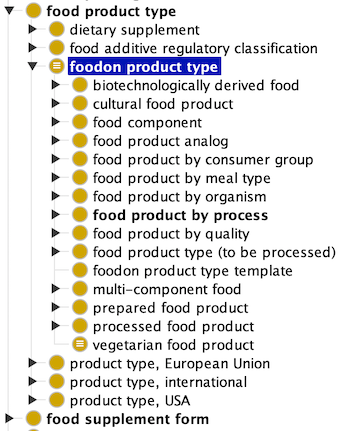
\includegraphics[width=10cm]{FIGURE/food_product_type.png}
	\end{center}
}
\caption{food product type}
\label{fig:food_product_type}
\end{figure}

\newpage

La classe ``\textbf{food transformation process}" � posizionata sotto la classe BFO ``\textbf{process}". Alcuni processi di FoodOn possono essere multiuso, ad esempio, il congelamento pu� essere per la conservazione degli alimenti o per produrre un effetto come nel gelato. Altri sono specifici per la conservazione o altri obiettivi del processo. \textit{(Figur \ref{fig:food_transformation_process})}
\begin{figure}[!h] {
	\begin{center}
		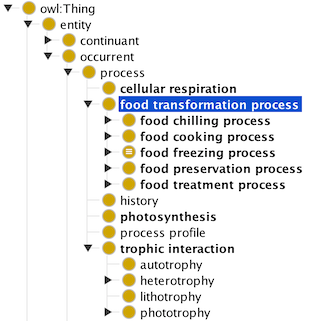
\includegraphics[width=10cm]{FIGURE/food_transformation_process.png}
	\end{center}
}
\caption{food transformation process}
\label{fig:food_transformation_process}
\end{figure}

\newpage

Sotto la classe ``\textbf{quality}" si trovano le qualit� osservabili del cibo come, ad esempio, la consistenza della carne del pesce o il colore della polpa o della buccia di un frutto. \textit{(Figur \ref{fig:foodon_quality})}\newline NB: C'� anche una classe BFO ``quality": le due non sono ancora unificate ontologicamente.
\begin{figure}[!h] {
	\begin{center}
		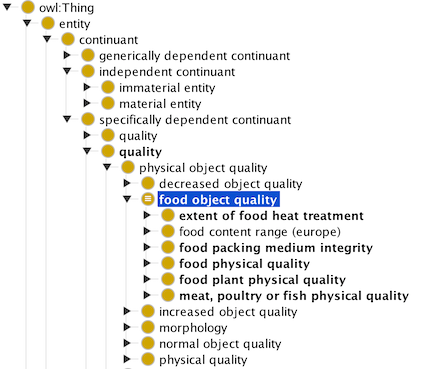
\includegraphics[width=10cm]{FIGURE/foodon_quality.png}
	\end{center}
}
\caption{quality}
\label{fig:foodon_quality}
\end{figure}

\newpage

Alcune categorie di informazioni che riguardano gli alimenti e che di solito non sono viste direttamente come qualit� di un prodotto alimentare, ma piuttosto sono informazioni pi� legate a fatti legislativi o affermazioni del produttore sull'articolo, di trovano in ``\textbf{information content entity}". \textit{(Figur \ref{fig:information_content_entity})}
\begin{figure}[!h] {
	\begin{center}
		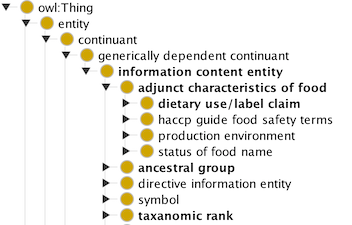
\includegraphics[width=10cm]{FIGURE/information_content_entity.png}
	\end{center}
}
\caption{information content entity}
\label{fig:information_content_entity}
\end{figure}
    
\section{Funzionalit�}
\index{Funzionalit�}

